%!TEX root = ./template-skripsi.tex
%-------------------------------------------------------------------------------
%                            	BAB IV
%               		KESIMPULAN DAN SARAN
%-------------------------------------------------------------------------------

\chapter{HASIL DAN UJI COBA}


\section{Spiral Kedua}		%SPIRAL 2
\subsection{Perencanaan}

\begin{figure}[H]
	\centering
	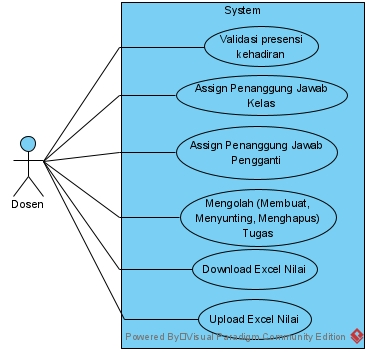
\includegraphics[width=0.8\textwidth]{gambar/diagram/Use Case Iteration 2}
	\caption{Desain \textit{Use Case Diagram Iterasi Kedua}}
	\label{fig:usecase2nd}
\end{figure}

	Dalam tahap perencanaan spiral 2, penulis kembali membuat desain\textit{ Use Case Diagram}, \textit{Activity Diagram}, dan rancangan tampilan antar muka yang akan menjadi tujuan pengembangan pada iterasi kedua. Pada spiral 2, penulis membuat halaman presensi, tugas, dan nilai untuk dosen. Fungsionalitas yang dibuat adalah memilih penanggung jawab, membuat tugas, menggunggah nilai, dan memvalidasi presensi kehadiran.  

\textbf{A. \textit{Use Case Diagram}}

	Pada Spiral 2, penambahan fitur dapat digambarkan dengan \textit{Use Case Diagram} pada gambar \ref{fig:usecase2nd}. Pada iterasi ini, pengembangan fitur berfokus kepada fungsionalitas pada \textit{user} Dosen seperti memilih penanggung jawab, membuat tugas, memvalidasi presensi kehadiran, dan mengunggah nilai.

\textbf{B. \textit{Activity Diagram}}

\begin{figure}[H]
	\centering
	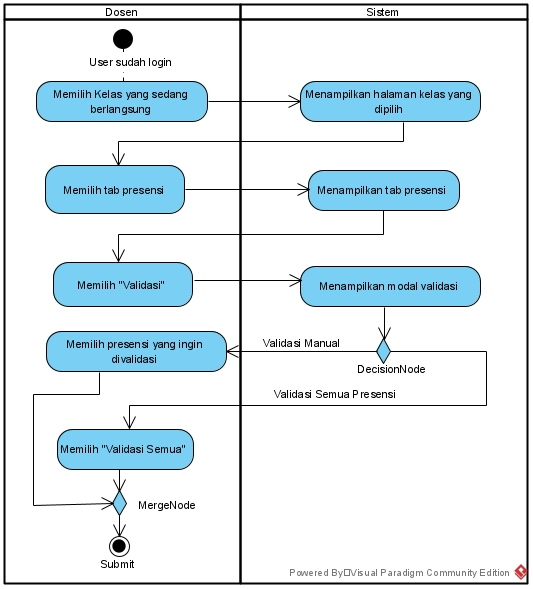
\includegraphics[width=0.8\textwidth]{gambar/diagram/Memvalidasi presensi}
	\caption{Desain \textit{Activity Diagram Memvalidasi Presensi}}
	\label{fig:actvalidasipresensi}
\end{figure}
	Dari beberapa \textit{Use Case} yang telah dibuat, penulis juga membuat \textit{Activty Diagram} untuk memperjelas alur cara kerja fitur yang dibuat. \textit{Activity Diagram} yang dibuat pada iterasi ini dapat dilihat pada gambar \ref{fig:actvalidasipresensi} dan gambar \ref{fig:acttugasnilai}

\begin{figure}[H]
	\centering
	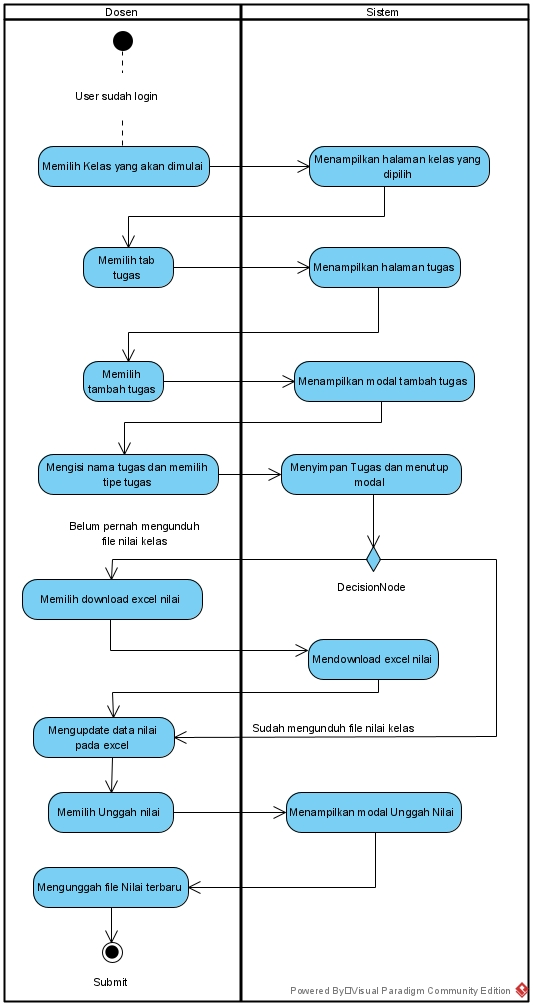
\includegraphics[width=0.8\textwidth]{gambar/diagram/Membuat tugas dan Mengunggah Nilai}
	\caption{Desain \textit{Activity Diagram Membuat tugas dan Mengunggah Nilai}}
	\label{fig:acttugasnilai}
\end{figure}


\textbf{C. Rancangan Tampilan Antar Muka}

	Pada Spiral 2, penulis juga membuat desain tampilan antar muka yang akan dibuat yaitu rancangan tampilan halaman Presensi, Tugas, dan Nilai. Pada gambar \ref{fig:mockpresensi} dapat dilihat desain tampilan halaman presensi dimana pengguna dapat melihat daftar mahasiswa yang mengikuti kelas dan presensi pada setiap pertemuannya. Pada gambar \ref{fig:mocktugas} dapat dilihat desain tampilan halaman tugas dimana dosen dapat membuat, menyunting, atau menghapus tugas. Pada tabel tugas, terdapat nama tugas, tanggal,  bobot, dan tipe. Bobot adalah bobot nilai tugas dalam persen sedangkan tipe adalah tipe tugas yang dapat berupa Tugas, UTS, atau UAS. Pada gambar \ref{fig:mocknilai} adalah desain tampilan halaman nilai yang hanya dapat dilihat oleh dosen. Pada tampilan ini dosen dapat mengunduh \textit{excel} nilai untuk mulai mengisi nilai, setelah \textit{file excel} sudah diisi dengan nilai, \textit{file} tersebut dapat diunggah kembali untuk memasukkan nilai ke dalam sistem.

\begin{figure}[h!]
	\centering
	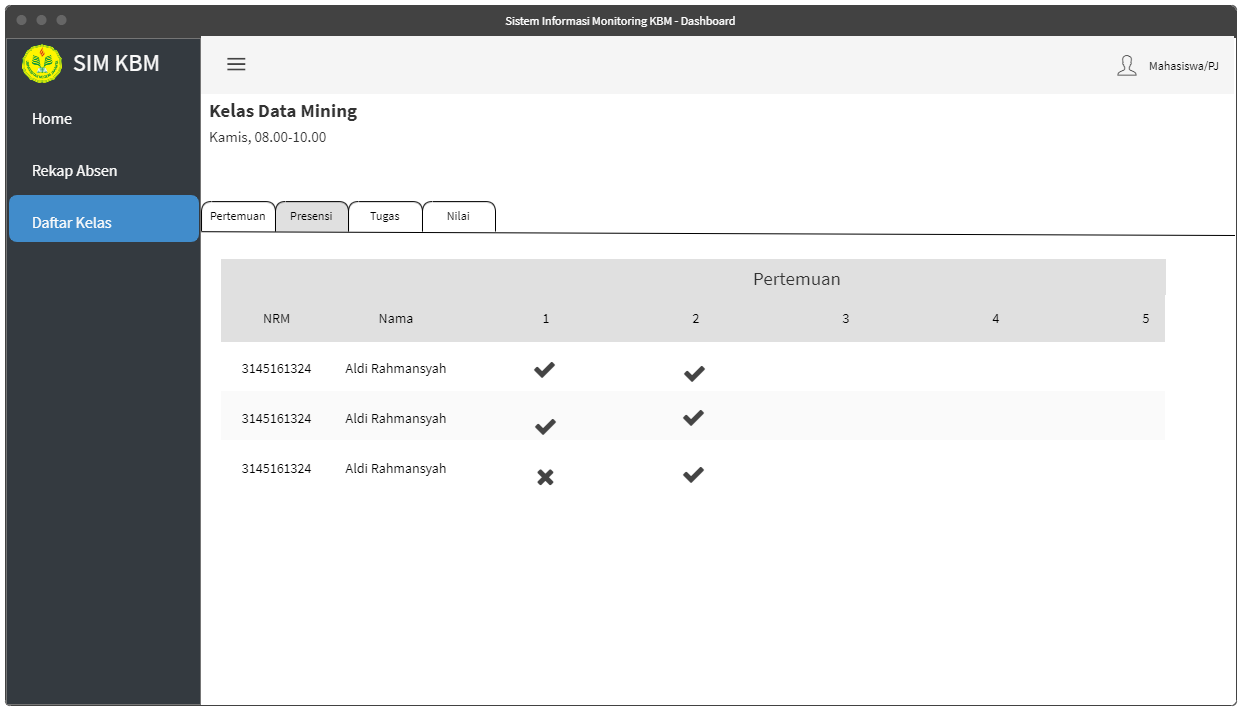
\includegraphics[width=1\textwidth]{gambar/mockup/form06_presensi}
	\caption{Desain Tampilan Halaman Presensi}
	\label{fig:mockpresensi}
\end{figure}

\begin{figure}[h!]
	\centering
	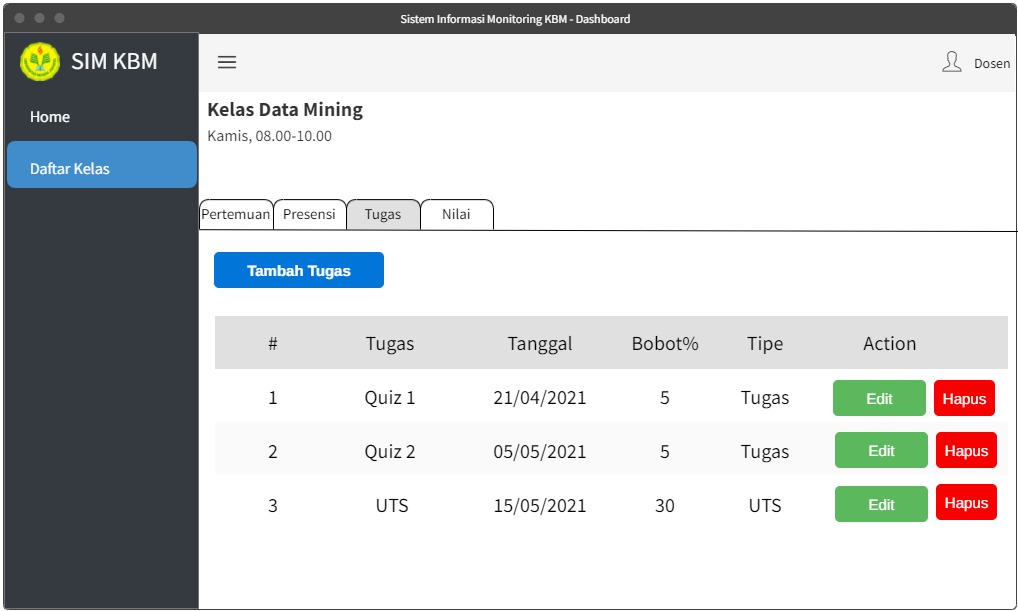
\includegraphics[width=1\textwidth]{gambar/mockup/tugas_dosen}
	\caption{Desain Tampilan Halaman Tugas Pada Dosen}
	\label{fig:mocktugas}
\end{figure}

\begin{figure}[h!]
	\centering
	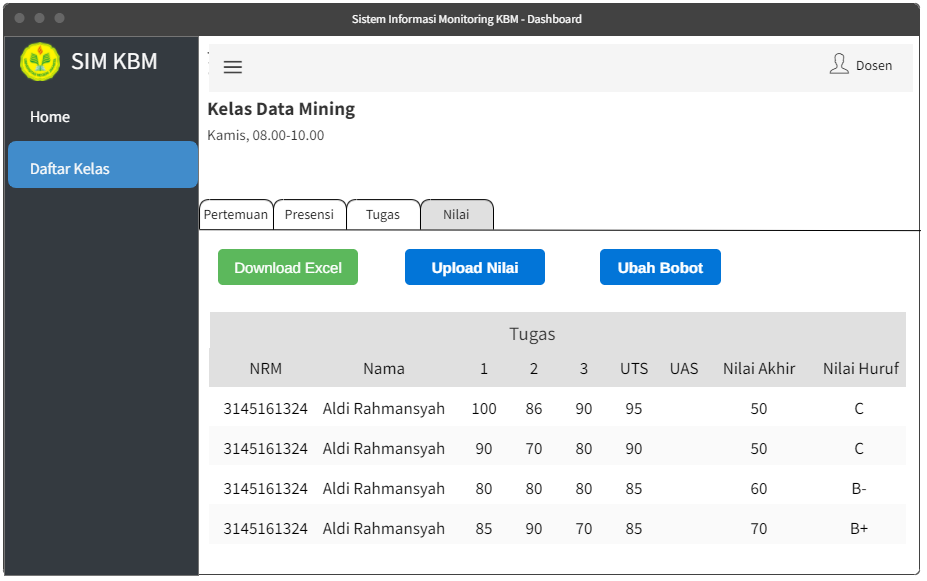
\includegraphics[width=1\textwidth]{gambar/mockup/nilai_dosen}
	\caption{Desain Tampilan Halaman Nilai Pada Dosen}
	\label{fig:mocknilai}
\end{figure}

\subsection{Analisis Risiko}
	Pada spiral 2, risiko yang didapati penulis ada pada membuat tampilan dan \textit{flow} yang sesuai dan dapat memberikan \textit{User Experience} yang terbaik.
\subsection{Pengembangan}
	Pada fase pengembangan, penulis melakukan proses pengembangan fitur-fitur yang telah direncanakan. Pada pengembangan spiral 2, penulis membuat tampilan halaman-halaman presensi, tugas, dan nilai pada \textit{frontend} dan membuat \textit{model} dan\textit{controller} pada \textit{backend}. Berikut adalah tampilan-tampilan yang telah dibuat pada fase pengembangan ini.

\begin{figure}[h!]
	\centering
	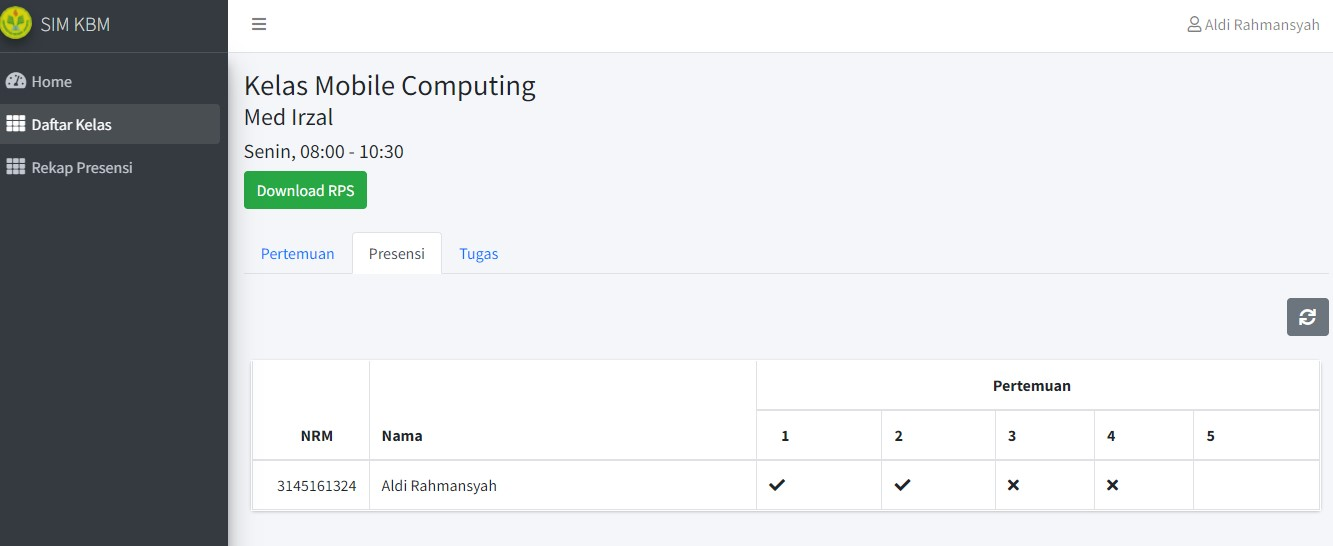
\includegraphics[width=1\textwidth]{gambar/ss/presensi}
	\caption{Tampilan Halaman Presensi}
	\label{fig:sspresensi}
\end{figure}

Pada gambar \ref{fig:sspresensi} adalah halaman \textit{tab} presensi atau form 06. Pada halaman ini terdapat tabel presensi yang berisi daftar mahasiswa dan presensi mahasiswa tersebut pada setiap pertemuan. Kehadiran mahasiswa akan ditandai dengan ikon centang sedangkan ketidakhadiran akan ditandai dengan ikon silang. Pada halaman presensi juga terdapat tombol \textit{reload} pada sisi kanan untuk memperbarui tabel jika ada perubahan.

\begin{figure}[h!]
	\centering
	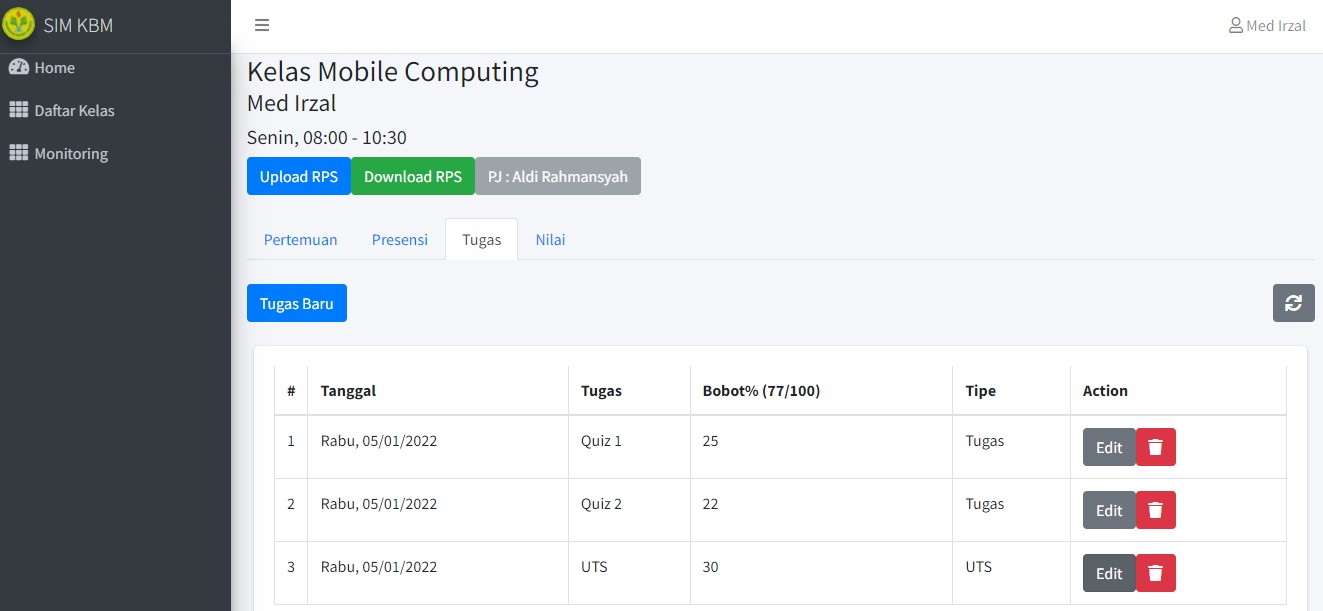
\includegraphics[width=1\textwidth]{gambar/ss/tugas}
	\caption{Tampilan Halaman Tugas Pada Dosen}
	\label{fig:sstugas}
\end{figure}

\begin{figure}[h!]
	\centering
	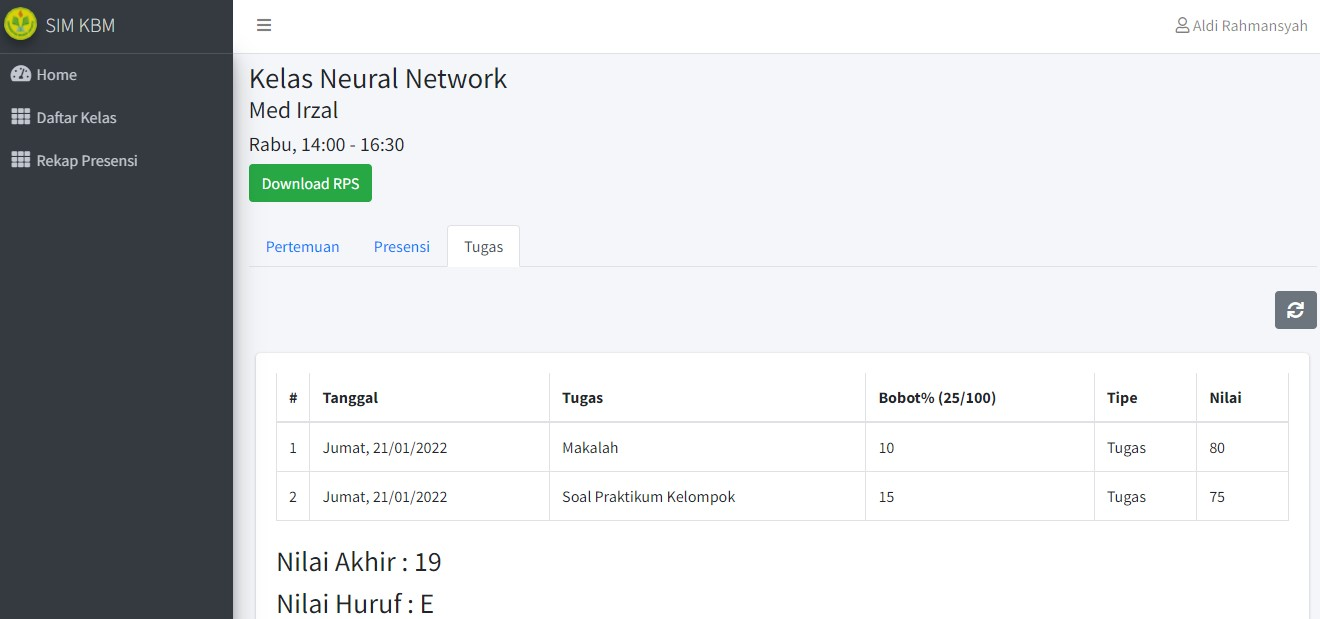
\includegraphics[width=1\textwidth]{gambar/ss/tugas_mhs}
	\caption{Tampilan Halaman Tugas Pada Mahasiswa}
	\label{fig:sstugasmhs}
\end{figure}

Pada gambar \ref{fig:sstugas} adalah halaman \textit{tab} tugas pada dosen dan gambar \ref{fig:sstugasmhs} adalah halaman \textit{tab} tugas pada mahasiswa. Pada halaman ini dosen dapat membuat tugas baru, menyunting, dan menghapus tugas yang sudah ada. Pada kolom bobot terdapat jumlah bobot tugas-tugas yang telah dibuat, jika bobot sudah mencapai 100 atau lebih, tulisan tersebut akan menjadi berwarna merah untuk menandakan bobot tugas sudah lengkap. Pada mahasiswa, halaman tugas akan berisi nilai pada masing-masing tugas, dan nilai akhir beserta nilai hurufnya. Pada halaman tugas juga terdapat tombol \textit{reload} pada sisi kanan untuk memperbarui tabel jika ada perubahan.

\begin{figure}[h!]
	\centering
	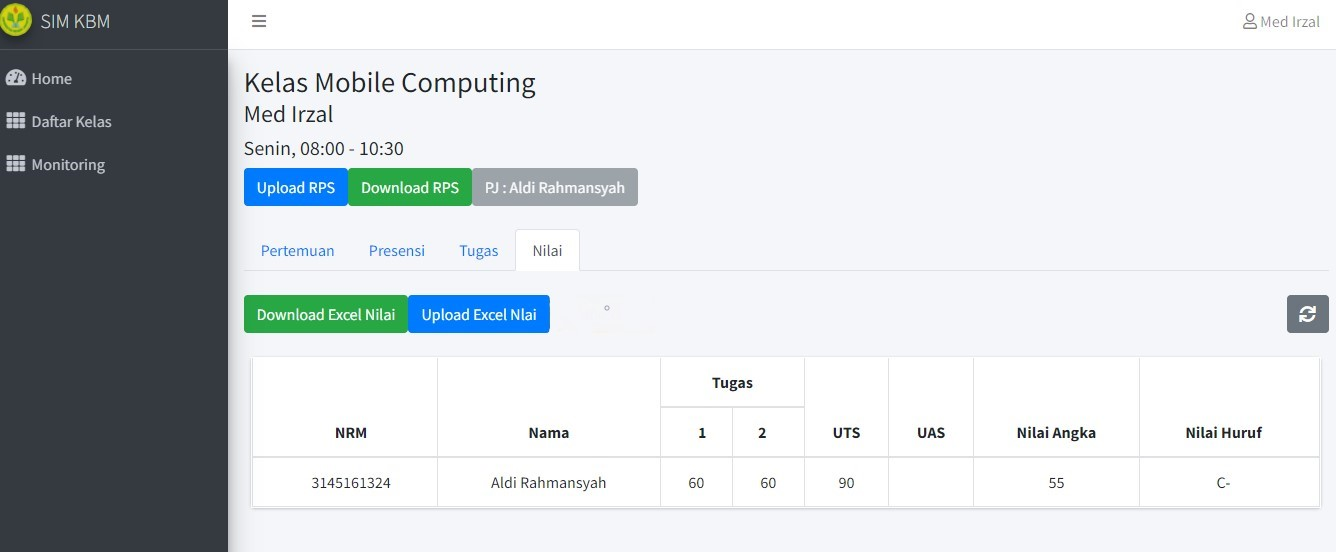
\includegraphics[width=1\textwidth]{gambar/ss/nilai}
	\caption{Tampilan Halaman Nilai}
	\label{fig:ssnilai}
\end{figure}

Pada gambar \ref{fig:ssnilai} adalah halaman \textit{tab} nilai yang hanya dapat dilihat oleh dosen. Pada halaman ini dosen dapat mengunggah dan mengunduh \textit{excel} nilai.

\subsection{Evaluasi}
	Pada fase evaluasi, penulis kembali melakukan pengujian kembali fitur yang telah dibuat dan melakukan \textit{review} pada kode yang telah dibuat untuk mencari cara implementasi yang lebih baik. Pada fitur nilai, dibutuhkan untuk menerapkan aturan \textit{input} nilai yaitu mahasiswa hanya bisa mendapatkan nilai UAS jika jumlah kehadiran mencapai 80\%. Pada iterasi selanjutnya penulis akan melanjutkan pengembangan dan memperbaiki fitur penanggung jawab pengganti menjadi khusus pada satu pertemuan saja.

\section{Spiral Ketiga}		%SPIRAL 3
\subsection{Perencanaan}
	Pada spiral 3, penulis merencanakan untuk memperbaiki fitur yang telah dievaluasi pada spiral sebelumnya dan menambahkan fitur-fitur baru yaitu menampilkan halaman monitoring untuk TPjM yang menampilkan data-data kelas yang ada dalam satu program studi, fitur unggah dan unduh RPS, rekap presensi mahasiswa, dan halaman admin untuk mengatur \textit{role} TPjM.

\textbf{A. \textit{Use Case Diagram}}

\begin{figure}[h!]
	\centering
	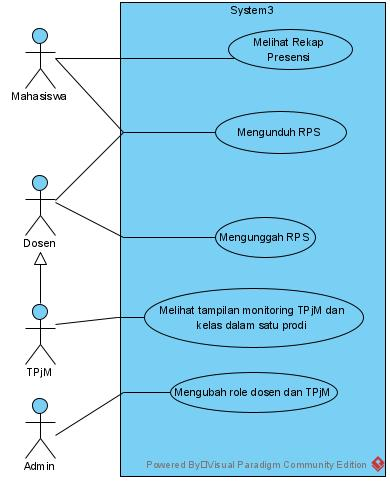
\includegraphics[width=0.8\textwidth]{gambar/diagram/Use Case Iteration 3}
	\caption{Desain \textit{Use Case Diagram Iterasi Ketiga}}
	\label{fig:usecase3rd}
\end{figure}

	Pada Spiral 3, penambahan fitur dapat digambarkan dengan \textit{Use Case Diagram} pada gambar \ref{fig:usecase3rd}. Pada iterasi ini, dilakukan pengembangan fitur pada beberapa aktor, pada mahasiswa ada penambahan rekap presensi dan mengunduh RPS, pada dosen terdapat penambahan mengunggah dan mengunduh RPS. Selain itu ditambahkan tampilan monitoring TPjM yang berupa daftar kelas dalam satu program studi yang merupakan \textit{homebase} dosen yang bersangkutan. Pada iterasi ini ditambahkan juga aktor baru yaitu admin yang memiliki fungsi untuk mengubah \textit{role} TPjM.


\textbf{B. \textit{Activity Diagram}}

	Pada spiral 3, penulis membuat \textit{Activity Diagram} untuk membantu menjelaskan interaksi yang terjadi pada \textit{Use Case}. \textit{Activity Diagram} yang dibuat pada iterasi ini dapat dilihat pada gambar \ref{fig:actadmin}.

\begin{figure}[h!]
	\centering
	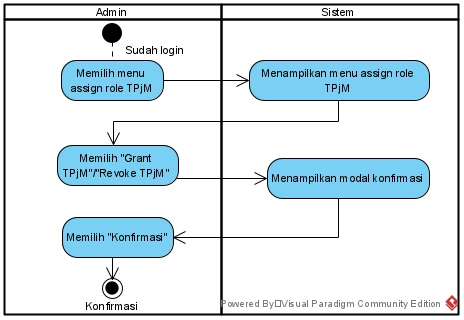
\includegraphics[width=0.8\textwidth]{gambar/diagram/Admin Assign Role}
	\caption{Desain \textit{Activity Diagram Admin Assign Role}}
	\label{fig:actadmin}
\end{figure}

\textbf{C. Rancangan Tampilan Antar Muka}

	Pada Spiral 2, penulis membuat desain tampilan antar muka yang akan dibuat yaitu rancangan tampilan halaman admin, rekap presensi, dan halaman monitoring. Pada gambar \ref{fig:mockadmin} dapat dilihat desain tampilan halaman dimana admin dapat mengganti \textit{role} dosen menjadi TPjM atau sebaliknya. Pada gambar \ref{fig:mockrekappresensi} dapat dilihat desain tampilan halaman rekap presensi mahasiswa. Pada gambar \ref{fig:mockmonitoring} dapat dilihat tampilan halaman monitoring dimana TPjM dapat melihat daftar kelas pada program studi \textit{homebase}nya.

\begin{figure}[h!]
	\centering
	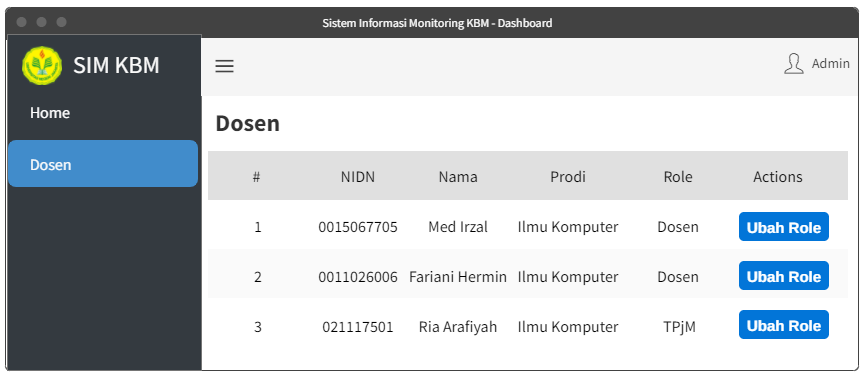
\includegraphics[width=1\textwidth]{gambar/mockup/admin_dosen}
	\caption{Desain Tampilan Halaman Admin \textit{Assign Role}}
	\label{fig:mockadmin}
\end{figure}

\begin{figure}[h!]
	\centering
	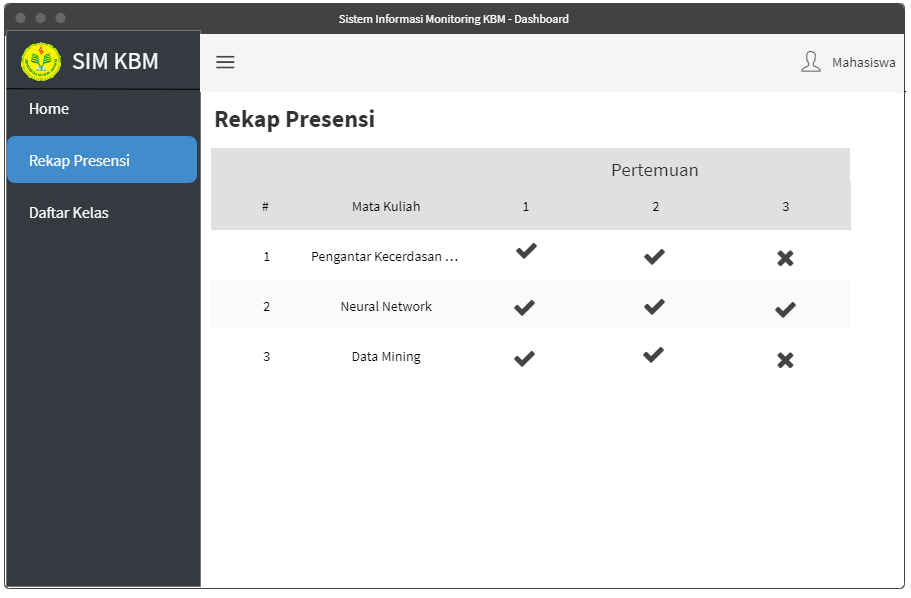
\includegraphics[width=1\textwidth]{gambar/mockup/rekap_presensi}
	\caption{Desain Tampilan Halaman Rekap Presensi}
	\label{fig:mockrekappresensi}
\end{figure}

\begin{figure}[h!]
	\centering
	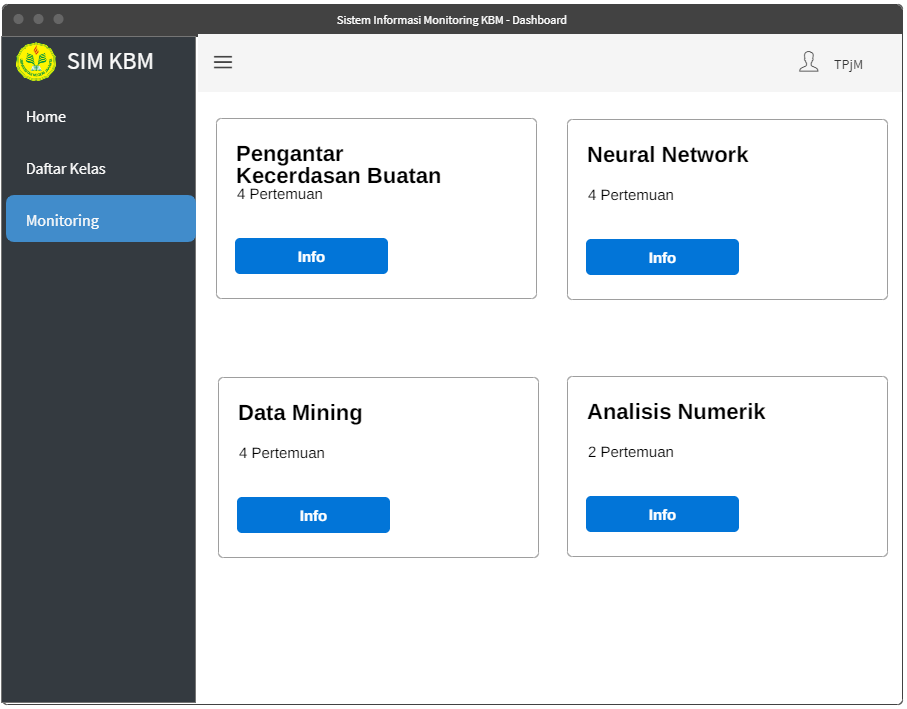
\includegraphics[width=1\textwidth]{gambar/mockup/monitoring}
	\caption{Desain Tampilan Halaman Monitoring}
	\label{fig:mockmonitoring}
\end{figure}

\subsection{Analisis Risiko}
	Pada fase ini, penulis mendapatkan hasil analisis yaitu dibutuhkan API SIAKAD tambahan untuk mengambil data semua kelas pada satu program studi dan membuat tampilan kelas tanpa adanya action apa-apa untuk tampilan monitoring TPjM.
\subsection{Pengembangan}
	Pada pengembangan spiral 3, penulis membuat tampilan daftar kelas monitoring TPjM dan rekap presensi dan pada \textit{backend} penulis membuat \textit{import export excel} untuk mengunduh dan mengunggah nilai. Berikut adalah tampilan-tampilan yang telah dibuat pada fase pengembangan ini.

\begin{figure}[h!]
	\centering
	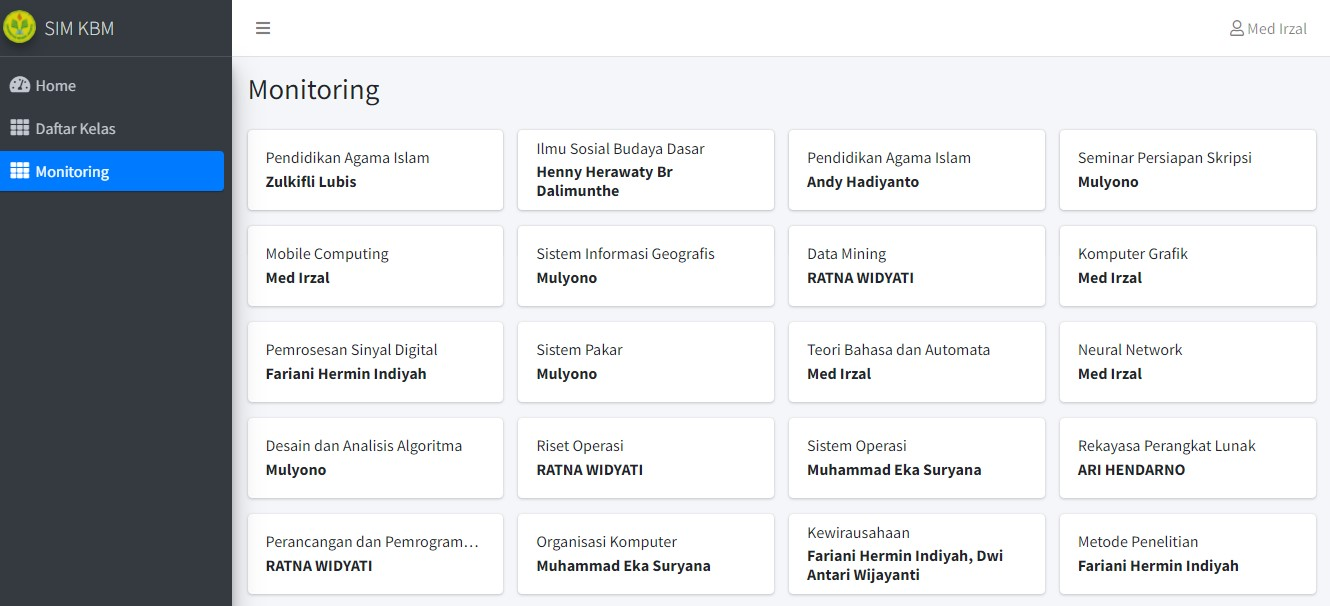
\includegraphics[width=1\textwidth]{gambar/ss/monitoring}
	\caption{Tampilan Halaman Monitoring}
	\label{fig:ssmonitoring}
\end{figure}

Pada gambar \ref{fig:ssmonitoring} adalah tampilan halaman monitoring dimana TPjM dapat melihat daftar kelas yang ada pada program studi, TPjM dapat mengeklik salah satu kelas untuk melihat halaman kelas tersebut. Halaman kelas yang dibuka dari menu monitoring tidak memiliki tombol interaksi apapun kecuali mengunduh RPS dan nilai.

\begin{figure}[h!]
	\centering
	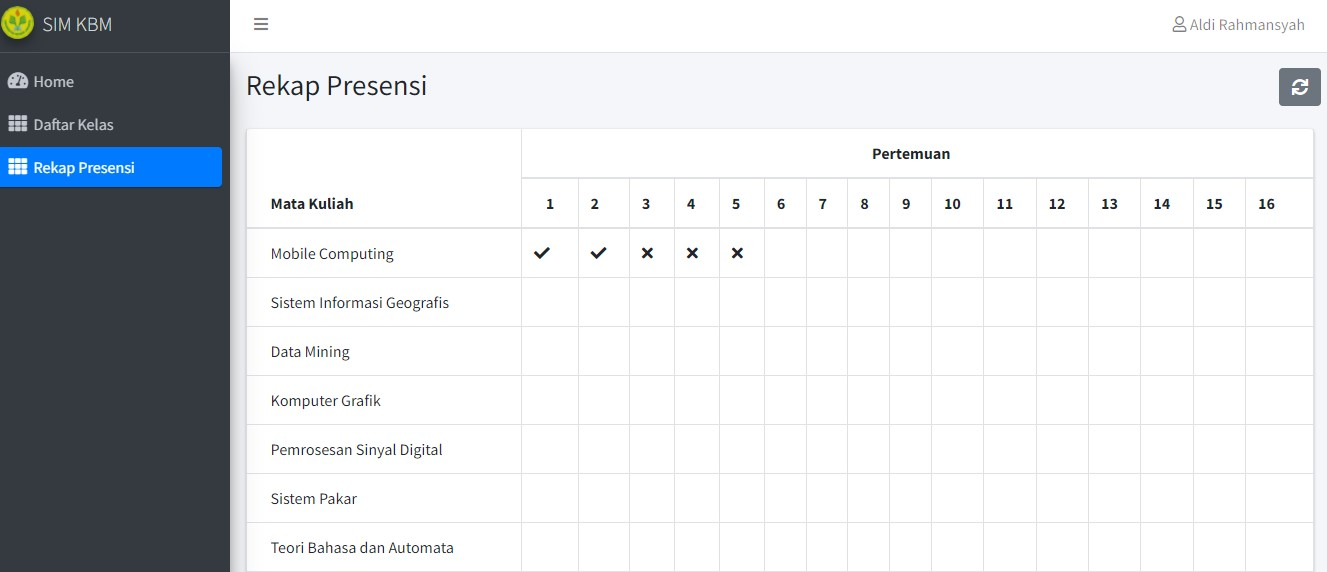
\includegraphics[width=1\textwidth]{gambar/ss/rekap_presensi}
	\caption{Tampilan Halaman Rekap Presensi}
	\label{fig:ssrekappresensi}
\end{figure}

\begin{figure}[h!]
	\centering
	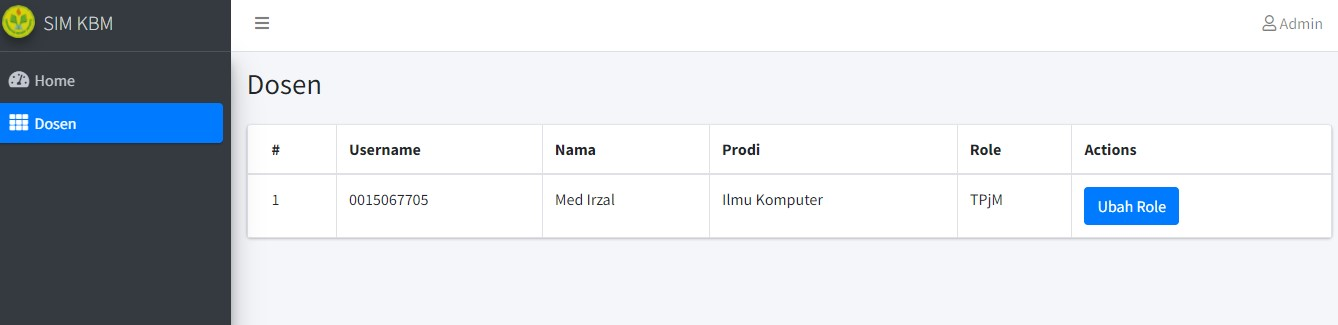
\includegraphics[width=1\textwidth]{gambar/ss/admin}
	\caption{Tampilan Halaman Admin}
	\label{fig:ssadmin}
\end{figure}

\subsection{Evaluasi}
	Pada evaluasi spiral 3, didapatkan kebutuhan untuk melihat data kelas pada semester sebelumnya baik pada mahasiswa, dosen, maupun monitoring. Penulis memutuskan untuk menambah iterasi tambahan untuk memperbaiki detil-detil fitur dan tampilan yang sudah ada dan beberapa perubahan desain dan kebutuhan.

\section{Spiral Keempat}		%SPIRAL 4
\subsection{Perencanaan}
	Pada fase perencanaan spiral 4, penulis menambahkan perizinan mahasiswa, mengubah bobot tugas sekaligus pada halaman nilai untuk mempermudah dosen, dan kebutuhan untuk melihat data pada semester sebelumnya. Selain itu penulis juga memperbaiki beberapa detil tampilan dan fitur-fitur lainnya.

\textbf{A. \textit{Use Case Diagram}}

	Pada spiral 4, penambahan pada i dapat dilihat pada gambar \ref{fig:usecase4th}. Pada gambar tersebut dapat dilihat penambahan \textit{Use Case} pada aktor dosen dan mahasiswa. 

\begin{figure}[h!]
	\centering
	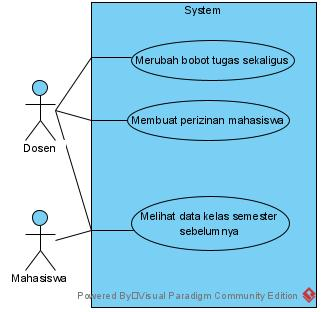
\includegraphics[width=0.8\textwidth]{gambar/diagram/Use Case Iteration 4}
	\caption{Desain \textit{Use Case Diagram Iterasi Keempat}}
	\label{fig:usecase4th}
\end{figure}

\textbf{B. \textit{Activity Diagram}}

	Pada spiral 4, penulis membuat \textit{Activity Diagram} untuk membantu menjelaskan interaksi yang terjadi pada \textit{Use Case}. \textit{Activity Diagram} yang dibuat pada iterasi ini dapat dilihat pada gambar \ref{fig:actperizinan}.

\begin{figure}[h!]
	\centering
	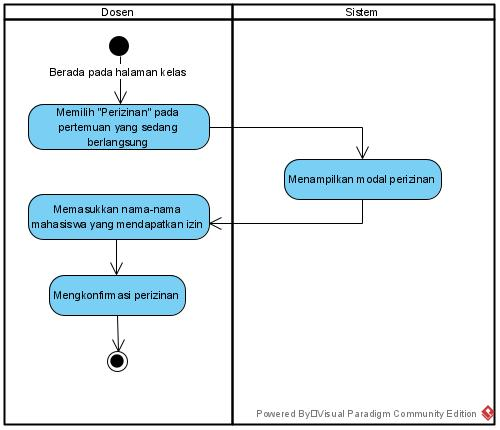
\includegraphics[width=0.8\textwidth]{gambar/diagram/perizinan}
	\caption{Desain \textit{Activity Diagram} Perizinan}
	\label{fig:actperizinan}
\end{figure}

\subsection{Analisis Risiko}
	Pada spiral 4, dikarenakan adanya kebutuhan baru untuk dapat melihat data semester sebelumnya, penulis harus melakukan perubahan pada kode yang sudah ada yang sebelumnya hanya memberikan data dengan semester aktif.
\subsection{Pengembangan}
	Pada pengembangan spiral 4, penulis menambahkan tombol perizinan pada halaman presensi dan tombol Ubah Bobot Tugas pada halaman nilai, untuk mengubah bobot tugas sekaligus untuk mempermudah dosen jika ingin menyesuaikan bobot tugas dan melihat efek perubahan bobot tugas tersebut pada nilai mahasiswa. Penulis juga menambahkan pemilihan semester pada rekap presensi, daftar kelas, dan monitoring untuk melihat data pada semester sebelumnya. 
\subsection{Evaluasi}
	Pada evaluasi spiral terakhir, penulis melakukan \textit{review} pada fitur-fitur yang sudah ada dan memastikan bahwa semuanya sudah berjalan dengan baik dan sesuai kebutuhan. Setelah semua fitur-fitur yang ada telah dievaluasi dan sudah berjalan sesuai dengan desain dan kebutuhan sistem siap untuk dilakukan pengujian oleh pengguna.
%END SPIRAL 


\section{Uji Coba}
	Uji coba pada sistem dilakukan terhadap enam responden mahasiswa yang pernah atau sedang menjadi penanggung jawab kelas dan empat dosen dimana tiga di antaranya merupakan TPjM. Setiap responden akan menguji coba sistem yang telah dikembangkan berdasarkan peran masing-masing responden. Uji coba yang dilakukan menggunakan data yang didapatkan dari hasil sebaran kuesioner \textit{User Acceptance Test}. \textit{User Acceptance Test} bertujuan untuk mengetahui apakah sistem yang dibuat sudah sesuai dengan kebutuhan \textit{user} atau belum. Berikut langkah-langkah pengujian yang akan dilakukan pada sistem informasi Koperasi Mahasiswa Universitas Negeri Jakarta:
\begin{enumerate}
	\item Mahasiswa
	\begin{itemize}
		\item Melakukan \textit{login} menggunakan akun SIAKAD.
		\item Mengunduh RPS.
		\item Membuat pertemuan.
		\item Memvalidasi pertemuan.
		\item Mengisi kehadiran pertemuan.
		\item Melihat data presensi kehadiran kelas.
		\item Melihat data tugas dan perhitungan nilai.
		\item Melihat rekap presensi.
		\item Melihat data semester sebelumnya.
	\end{itemize}
	\item Dosen
	\begin{itemize}
		\item Melakukan \textit{login} menggunakan akun SIAKAD.
		\item Mengolah (membuat, menyunting, menghapus) pertemuan.
		\item Memvalidasi pertemuan.
		\item Memvalidasi presensi kehadiran.
		\item Mengisi perizinan mahasiswa.
		\item Melihat data presensi kehadiran kelas.
		\item Mengolah (membuat, menyunting, menghapus) tugas.
		\item Mengunduh dan mengunggah \textit{excel} nilai.
		\item Memilih penanggung jawab kelas dan penanggung jawab sementara.
		\item Mengunggah dan mengunduh RPS.
		\item Melihat halaman monitoring untuk TPjM.
		\item Melihat data semester sebelumnya.
	\end{itemize}
\end{enumerate}

Pengujian yang dilakukan terdiri dari dua pengujian, yaitu pengujian fungsionalitas dan pengujian kebergunaan atau \textit{usablity}. Pada pengujian fungsional, sistem penilaian yang digunakan berdasarkan pada pilihan: \\

\begin{tabular}{lll}
S& : Setuju\\
TS& : Tidak Setuju\\
\\
\end{tabular}

Pada pengujian kebergunaan (\textit{usability}), sistem penilaian yang digunakan adalah skala likert. Skala likert adalah skala yang terdiri dari serangkaian pernyataan yang menjelaskan sikap responden terhadap objek penelitian. Setiap pernyataan terdapat lima poin dari skala "sangat tidak setuju" hingga "sangat tidak setuju" \citep{Ahyar2020}. Setelah didapatkan seluruh data penilaian dari responden, nilai tersebut dikalkulasikan sesuai sistem penilaian berikut:

\begin{itemize}
	\item Nilai Total

		Nilai total adalah jumlah keseluruhan yang didadapat dari tiap pernyataan atau dapat ditulis menjadi: \\
		\(Nilai Total = (jumlah \times skorSS) + (jumlah \times skorS) + (jumlah \times skorC) + (jumlah \times skorTS) + (jumlah \times skorSTS)\)
	\item Persentase Kelayakan
		Persentase kelayakan adalah persentase nilai rata-rata yang didapatkan dengan cara membagi nilai total dengan skor maksimal.  Skor maksimal adalah nilai maksimal skala likert yang dikalikan dengan jumlah pernyataan. Perhitungan tersebut dapat ditulis menjadi: \\
		\(Persentase Kelayakan(\%) = \frac{NilaiTotal}{SkorMaksimal}\times100\)
\end{itemize}

Persentase kelayakan yang sudah didapatkan akan dibandingkan dengan skor pada skala likert untuk menarik kesimpulan akhir dari hasil pengujian. Berikut model skor skala likert:\\

\begin{tabular}{lll}
1. Sangat Kurang Sesuai& = 0\% - 20\%\\
2. Kurang Sesuai& = 21\% - 40\%\\
3. Cukup Sesuai& = 41\% - 60\%\\
4. Sesuai& = 61\% - 80\%\\
5. Sangat Sesuai& = 81\% - 100\%\\
\\
\end{tabular}

\section{Hasil Uji Coba}
Berdasarkan hasil uji coba \textit{User Acceptance Test} yang dilakukan terhadap enam responden mahasiswa dan empat responden dosen, diperoleh hasil uji coba sebagai berikut:

\subsection{Pengujian Oleh Mahasiswa}
Pengujian oleh mahasiswa dilakukan oleh enam mahasiswa yang mencakup empat mahasiswa program studi Ilmu Komputer dan dua mahasiswa pendidikan matematika . Berikut merupakan hasil penilaian \textit{User Acceptance Test} yang diberikan Mahasiswa mengenai fungsionalitas dan kebergunaan:

\begin{table}[h!]
\centering
\def\arraystretch{1.5}
\caption{Hasil Uji Fungsionalitas Pada Mahasiswa}
\label{tab:fungsiomhs}
\begin{tabular} { | >{\centering\arraybackslash}m{1em} | >{\raggedright\arraybackslash}m{22em} | >{\centering\arraybackslash}m{3.7em} | >{\centering\arraybackslash}m{3.7em} | }
	\hline
	\multirow{2}{*}{\textbf{No.}} & \multicolumn{1}{c|}{\multirow{2}{*}{\textbf{Pernyataan}}} & \multicolumn{2}{c|}{\textbf{Jawaban Responden}} \\ 
	\cline{3-4} && \textbf{TS} & \textbf{S}\\
	\hline

	1 & Fitur \textit{login} berjalan dengan baik. & 0 & 6 \\ \hline
	2 & Fitur daftar kelas dan filter semester berjalan dengan baik. & 0 & 6 \\ \hline
	3 & Fitur mengunduh rps berjalan dengan baik. & 0 & 6 \\ \hline
	4 & Fitur mengelola (membuat dan memvalidasi) pertemuan berjalan dengan baik. & 0 & 6 \\ \hline
	5 & Fitur hadir dan validasi presensi berjalan dengan baik. & 0 & 6 \\ \hline
	6 & Fitur tabel presensi berjalan dengan baik. & 0 & 6 \\ \hline
	7 & Fitur tugas dan nilai berjalan dengan baik. & 0 & 6 \\ \hline
	8 & Fitur rekap presensi dan filter semester berjalan dengan baik. & 0 & 6 \\ \hline
	9 & Fitur \textit{logout} berjalan dengan baik. & 0 & 6 \\ \hline
	\multicolumn{2}{|c|}{Total} & 0 & 54 \\ \hline
	\multicolumn{2}{|c|}{Persentase Jawaban} & \textbf{0\%} & \textbf{100\%} \\ \hline

\end{tabular}
\end{table}

Berdasarkan hasil uji coba fungsionalitas dari kuisioner UAT pada pengguna mahasiswa, didapatkan persentase jawaban sebesar 100\%. Dari hasil persentase jawaban yang didapatkan, dapat dikatakan bahwa sistem informasi monitoring kegiatan belajar mengajar ini berjalan dengan baik dan sesuai dengan yang diharapkan.

%\begin{table}[h!]
%\centering
%\def\arraystretch{1.5}

\begin{longtable}[h!] { | >{\centering\arraybackslash}m{1em} | >{\raggedright\arraybackslash}m{22em} | >{\centering\arraybackslash}m{1em} | >{\centering\arraybackslash}m{1em} | >{\centering\arraybackslash}m{1em} | >{\centering\arraybackslash}m{1em} | >{\centering\arraybackslash}m{1em} | }
\caption{Hasil Uji Kebergunaan Pada Mahasiswa}
\label{tab:usabilmhs}\\
	\hline
	\multirow{2}{*}{\textbf{No.}} & \multicolumn{1}{c|}{\multirow{2}{*}{\textbf{Pernyataan}}} & \multicolumn{5}{c|}{\textbf{Jawaban Responden}} \\ 
	\cline{3-7} && \textbf{1} & \textbf{2} & \textbf{3} & \textbf{4} & \textbf{5}\\
	\hline

	1 & Fitur hadir dan validasi presensi mudah dimengerti. & 0 & 0 & 0 & 1 & 5 \\ \hline
	2 & Fitur mengelola (membuat dan memvalidasi) pertemuan mudah dimengerti. & 0 & 0 & 1 & 1 & 4 \\ \hline
	3 & Fitur rekap presensi dan filter semester mudah dimengerti. & 0 & 0 & 0 & 1 & 5 \\ \hline
	4 & Sistem ini mudah digunakan. & 0 & 0 & 0 & 1 & 5 \\ \hline
	5 & Sistem ini nyaman digunakan. & 0 & 0 & 0 & 2 & 4 \\ \hline
	6 & Sistem ini dapat membantu mahasiswa dalam proses kegiatan belajar mengajar. & 0 & 0 & 0 & 1 & 5 \\ \hline
	\multicolumn{2}{|c|}{Total} & 0 & 0 & 1 & 7 & 28 \\ \hline

\end{longtable}
%\end{table}

\(Nilai Total = (0 \times 1) + (0 \times 2) + (1 \times 3) + (7 \times 4) + (28 \times 5) = 171\).
\indent \(Persentase Kelayakan(\%) = \frac{171}{180}\times100=95\%\). \\
\indent Berdasarkan hasil uji coba kebergunaan pada pengguna mahasiswa, didapatkan persentase kelayakan senilai 95\%. Dari hasil persentase kelayakan yang didapatkan, dapat dikatakan bahwa sistem informasi monitoring kegiatan belajar mengajar ini mendapat predikat sesuai dalam aspek kebergunaan sistem.

\subsection{Pengujian Oleh Dosen}
Pengujian oleh dosen dilakukan oleh empat dosen dari masing-masing program studi Ilmu Komputer, Pendidikan Matematika, Matematika, dan Statistika dimana tiga diantaranya merupakan TPjM. Berikut merupakan hasil penilaian \textit{User Acceptance Test} yang diberikan dosen mengenai fungsionalitas dan kebergunaan:

%\begin{table}[h!]
%\centering
%\def\arraystretch{1.5}
\begin{longtable} { | >{\centering\arraybackslash}m{1em} | >{\raggedright\arraybackslash}m{22em} | >{\centering\arraybackslash}m{3.7em} | >{\centering\arraybackslash}m{3.7em} | }
\caption{Hasil Uji Fungsionalitas Pada Dosen}
\label{tab:fungsiodsn} \\
	\hline
	\multirow{2}{*}{\textbf{No.}} & \multicolumn{1}{c|}{\multirow{2}{*}{\textbf{Pernyataan}}} & \multicolumn{2}{c|}{\textbf{Jawaban Responden}} \\ 
	\cline{3-4} && \textbf{TS} & \textbf{S}\\
	\hline

	1 & Fitur login berjalan dengan baik. & 0 & 4 \\ \hline
	2 & Fitur daftar kelas dan filter semester berjalan dengan baik. & 0 & 4 \\ \hline
	3 & Fitur unggah dan unduh RPS berjalan dengan baik. & 0 & 4 \\ \hline
	4 & Fitur pilih penanggung jawab dan penanggung jawab sementara berjalan dengan baik. & 0 & 4 \\ \hline
	5 & Fitur mengelola (membuat, mengubah materi, memvalidasi, dan menghapus) pertemuan berjalan dengan baik. & 0 & 4 \\ \hline
	6 & Fitur tabel presensi berjalan dengan baik. & 0 & 4 \\ \hline
	7 & Fitur validasi  presensi dan perizinan berjalan dengan baik. & 0 & 4 \\ \hline
	8 & Fitur mengelola (membuat, mengyunting, dan menghapus) tugas berjalan dengan baik. & 0 & 4 \\ \hline
	9 & Fitur mengunggah dan mengunduh nilai berjalan dengan baik. & 0 & 4 \\ \hline
	10 & Fitur monitoring dan filter semester berjalan dengan baik (TPjM). & 0 & 3 \\ \hline
	11 & Fitur logout berjalan dengan baik. & 0 & 4 \\ \hline
	\multicolumn{2}{|c|}{Total} & 0 & 43 \\ \hline
	\multicolumn{2}{|c|}{Persentase Jawaban} & \textbf{0\%} & \textbf{100\%} \\ \hline

\end{longtable}
%\end{table}

Berdasarkan hasil uji coba fungsionalitas dari kuisioner UAT pada pengguna dosen, didapatkan persentase jawaban sebesar 100\%. Dari hasil persentase jawaban yang didapatkan, dapat dikatakan bahwa sistem informasi monitoring kegiatan belajar mengajar ini berjalan dengan baik dan sesuai dengan yang diharapkan.

%\begin{table}[H]
%\centering
\begin{longtable}[H] { | >{\centering\arraybackslash}m{1em} | >{\raggedright\arraybackslash}m{22em} | >{\centering\arraybackslash}m{1em} | >{\centering\arraybackslash}m{1em} | >{\centering\arraybackslash}m{1em} | >{\centering\arraybackslash}m{1em} | >{\centering\arraybackslash}m{1em} | }
\caption{Hasil Uji Kebergunaan Pada Dosen}
\label{tab:usabildsn} \\
	\hline
	\multirow{2}{*}{\textbf{No.}} & \multicolumn{1}{c|}{\multirow{2}{*}{\textbf{Pernyataan}}} & \multicolumn{5}{c|}{\textbf{Jawaban Responden}} \\ 
	\cline{3-7} && \textbf{1} & \textbf{2} & \textbf{3} & \textbf{4} & \textbf{5}\\
	\hline

	1 & Fitur upload dan download RPS mudah dimengerti. & 0 & 0 & 1 & 1 & 2 \\ \hline
	2 & Fitur pilih penanggung jawab dan penanggung jawab sementara mudah dimengerti. & 0 & 0 & 0 & 2 & 2 \\ \hline
	3 & Fitur mengelola (membuat, mengubah materi, memvalidasi, dan menghapus) pertemuan mudah dimengerti. & 0 & 0 & 0 & 3 & 1 \\ \hline
	4 & Fitur validasi  presensi dan perizinan mudah dimengerti. & 0 & 0 & 0 & 3 & 1 \\ \hline
	5 & Fitur mengelola (membuat, mengyunting, dan menghapus) tugas mudah dimengerti. & 0 & 0 & 0 & 3 & 1 \\ \hline
	6 & Fitur upload dan download nilai mudah dimengerti. & 0 & 0 & 0 & 2 & 2 \\ \hline
	7 & Sistem ini mudah digunakan. & 0 & 0 & 0 & 1 & 3 \\ \hline
	8 & Sistem ini nyaman digunakan. & 0 & 0 & 0 & 2 & 2 \\ \hline
	9 & Sistem ini dapat membantu dosen dalam proses kegiatan belajar mengajar & 0 & 0 & 0 & 2 & 2 \\ \hline
	10 & Sistem ini dapat membantu TPjM dalam melakukan monitoring evaluasi kegiatan belajar mengajar (TPjM) & 0 & 0 & 0 & 1 & 2 \\ \hline
	\multicolumn{2}{|c|}{Total} & 0 & 0 & 1 & 20 & 18 \\ \hline

\end{longtable}
%\end{table}

\(Nilai Total = (0 \times 1) + (0 \times 2) + (1 \times 3) + (20 \times 4) + (18 \times 5) = 173\).
\indent \(Persentase Kelayakan(\%) = \frac{173}{195}\times100=88.7\%\). \\
\indent Berdasarkan hasil uji coba kebergunaan pada pengguna dosen, didapatkan persentase kelayakan senilai 88.7\%. Dari hasil persentase kelayakan yang didapatkan, dapat dikatakan bahwa sistem informasi monitoring kegiatan belajar mengajar ini mendapat predikat sesuai dalam aspek kebergunaan sistem.

\subsection{Hasil Pengujian Keseluruhan Sistem}

Berdasarkan hasil pengujian fungsional pada kedua pengguna didapatkan didapatkan bahwa fitur-fitur yang terdapat pada sistem dapat berjalan dengan baik dengan penilaian dari kedua pengguna senilai 100\%. Selain itu didapatkan persentase kelayakan pada pengujian kebergunaan adalah sebagai berikut.

\begin{itemize}
	\item \textit{User} Mahasiswa \indent : 95\%
	\item \textit{User} Dosen \indent : 88.7\%
\end{itemize}

Dari persentase kedua pengguna kemudian dihitung total persentase kelayakan yang merupakan rata-rata dari kedua nilai persentase kelayakan tersebut. Sehingga total persentase yang didapatkan dapat dihitung sebagai berikut: \\
\indent \(Total Persentase Kelayakan(\%) = \frac{95\%+88.7\%}{2}=91.8\%\). \\
Berdasarkan hasil perhitungan tersebut, didapatkan total persentase kelayakan senilai 91.8\%. Total persentase kelayakan tersebut berada pada rentang 81\%-100\% yang berarti dapat dikatakan bahwa nilai kebergunaan keseluruhan sistem mendapatkan predikat sangat sesuai.






% Baris ini digunakan untuk membantu dalam melakukan sitasi
% Karena diapit dengan comment, maka baris ini akan diabaikan
% oleh compiler LaTeX.
\begin{comment}
\bibliography{daftar-pustaka}
\end{comment}